% ====================================================================
% v7-03.tex — graphite_ica_ch1 v7 (sub-agent v7-03)
%   흑연 음극 dQ/dV ICA 이론 — Chapter 1
%   절 순서 = v11_final 코드 진행 N0–N9 (플로우차트 spine 준수)
%   스타일   = v5 수식-구동 형식 (v6 참조 금지)
%   build: xelatex -interaction=nonstopmode (2-pass)
% ====================================================================
\documentclass[11pt,a4paper]{article}
\usepackage[margin=22mm]{geometry}
\usepackage{kotex}
\setmonofont{D2Coding}[Scale=MatchLowercase]
\usepackage{amsmath,amssymb,mathtools,bm}
\usepackage{booktabs,longtable,array}
\usepackage{enumitem}
\usepackage{amsthm}
\usepackage{hyperref}
\usepackage{fancyhdr}
\usepackage{lastpage}
\usepackage{setspace}
\usepackage{tikz}
\usetikzlibrary{positioning,arrows.meta}
\setstretch{1.12}
\setlength{\parskip}{0.45em}
\setlength{\parindent}{0pt}
\setlength{\headheight}{14pt}
\setlength{\emergencystretch}{2em}

\hypersetup{colorlinks=true, linkcolor=blue, urlcolor=blue, citecolor=blue,
  pdftitle={흑연 음극 dQ/dV 이론 — Chapter 1 (v7-03)}}
\pagestyle{fancy}\fancyhf{}
\lhead{흑연 음극 $\mathrm{d}Q/\mathrm{d}V$ 이론 — Ch.1 (v7-03, 수식-구동)}
\rhead{\thepage/\pageref{LastPage}}
\renewcommand{\headrulewidth}{0.4pt}

\newtheorem*{keybox}{핵심}
\newtheorem*{verifybox}{검산}

\newcommand{\dd}{\mathrm{d}}
\newcommand{\eff}{\mathrm{eff}}
\newcommand{\eq}{\mathrm{eq}}
\newcommand{\app}{\mathrm{app}}
\newcommand{\cell}{\mathrm{cell}}
\newcommand{\bg}{\mathrm{bg}}
\newcommand{\hys}{\mathrm{hys}}
\newcommand{\dis}{\mathrm{dis}}
\newcommand{\chg}{\mathrm{chg}}
\newcommand{\peak}{\mathrm{peak}}

\renewcommand{\theequation}{1.\arabic{equation}}
\renewcommand{\thesection}{1.\arabic{section}}

\title{\textbf{\LARGE Chapter 1}\\[0.4em]
  \Large 흑연 음극 $\mathrm{d}Q/\mathrm{d}V$ 이론:\\
  코드 진행 N0--N9 를 따라가는 수식-구동판 (v7-03)}
\author{}
\date{}

\makeatletter
\renewcommand*\l@section[2]{%
  \ifnum\c@tocdepth>\z@
    \addpenalty\@secpenalty
    \addvspace{1.0em\@plus\p@}
    \setlength\@tempdima{2.3em}
    \begingroup
      \parindent\z@\rightskip\@pnumwidth
      \parfillskip-\@pnumwidth
      \leavevmode\bfseries
      \advance\leftskip\@tempdima
      \hskip-\leftskip
      #1\nobreak\hfil\nobreak\hb@xt@\@pnumwidth{\hss#2\kern-\p@\kern\p@}\par
    \endgroup
  \fi}
\renewcommand*\l@subsection{\@dottedtocline{2}{2.3em}{3.2em}}
\makeatother

% ====================================================================
\begin{document}
\maketitle

% ====================================================================
\section*{서론}
\addcontentsline{toc}{section}{서론}
% ====================================================================

리튬이온전지 흑연 음극의 incremental capacity analysis(ICA)는 충방전 곡선 $Q(V)$ 의
미분 $\dd Q/\dd V$ 를 분석한다. 흑연은 stage $4\!\to\!3\!\to\!2\mathrm{L}\!\to\!2\!\to\!1$ 상전이를
거치며, 각 전이 전위에서 두 상이 공존하는 동안 전위가 거의 평탄해($\dd V/\dd q\to0$)
좁은 전위 구간에 큰 $\dd Q$ 가 집중되어 $\dd Q/\dd V$ 가 치솟는다. 이 peak 의
\textbf{위치·너비·높이}가 온도·C-rate·방향에 따라 어떻게 달라지는지를 하나의
물리식 사슬로 유도하는 것이 본 장의 목표다.

본 절의 구성은 \texttt{Anode\_Fit\_v11\_final.py} 의 핵심 메서드 \texttt{dqdv()}
가 계산을 진행하는 순서(N0$\to$N9)와 1:1 대응한다. 각 절이 한 노드의
물리식을 유도하고, 코드 식별자·부호를 그대로 따른다.

\tableofcontents
\newpage

% ====================================================================
\section{기호와 규약 (N0: 실험조건 $\to$ 모델 입력)}\label{sec:notation}
% ====================================================================

\texttt{curve()} facade 는 실험조건 $(V_\app,\,\text{direction},\,\text{c\_rate},\,
Q_\cell,\,T)$ 를 받아 \texttt{dqdv()} 코어로 넘긴다. 진입 과정에서 세 변환이 일어난다.

\paragraph{방향 부호.}
방전(\texttt{"discharge"}) $\to$ $\sigma_d=+1$, 충전(\texttt{"charge"}) $\to$
$\sigma_d=-1$ (\texttt{\_direction\_to\_sigma}, L514).

\paragraph{전류 크기.}
C-rate 를 절대 전류로 환산하면:
\begin{equation}
|I| = \text{c\_rate}\times Q_\cell \qquad [\mathrm{C/s}].
\label{eq:iabs}
\end{equation}

\paragraph{무차원 용량 좌표.}
$q = \int|I|\,\dd t\,/\,Q_\cell$ (방전 가지 기준). 본 문건이 뽑는 산출물은
$\dd Q/\dd V$ 이며, 이 미분은 \S\ref{sec:eqpeak} 에서 닫힌 해를 얻는다.

아래 표는 v11 코드와 본 문건 전개에서 등장하는 모든 기호를 코드 진행 순서로
정리한 것이다.

\begin{longtable}{p{0.16\textwidth} p{0.13\textwidth} p{0.63\textwidth}}
\toprule 기호 & 단위 & 의미 \\ \midrule \endhead
\multicolumn{3}{l}{\emph{--- 실험 입력(N0) ---}}\\
$V_\app$ & V & 인가(측정) 전위\\
$\sigma_d$ & --- & 방향 부호 (방전 $+1$ / 충전 $-1$)\\
$|I|$ & C/s & 전류 크기 $=\text{c\_rate}\cdot Q_\cell$\\
$T$ & K & 온도 (스칼라 또는 $V$ 배열)\\
$Q_\cell$ & C & 셀 총 방전 용량\\
$q$ & --- & 무차원 용량 $=\int|I|\dd t/Q_\cell$\\
\multicolumn{3}{l}{\emph{--- 분극(N1) ---}}\\
$V_n$ & V & 내부(열역학) 전위: $V_n = V_\app - \sigma_d|I|R_n$\\
$R_n$ & $\Omega$ & lumped 분극 저항 (\texttt{Rn})\\
\multicolumn{3}{l}{\emph{--- 평형 중심(N2) ---}}\\
$U_j(T)$ & V & 전이 $j$ 의 평형 전위\\
$\Delta H_{\mathrm{rxn},j}$ & J/mol & 삽입 반응 엔탈피 (\texttt{dH\_rxn})\\
$\Delta S_{\mathrm{rxn},j}$ & J/(mol\,K) & 삽입 반응 엔트로피 (\texttt{dS\_rxn})\\
$F$ & C/mol & Faraday 상수 ($96485$)\\
\multicolumn{3}{l}{\emph{--- 히스테리시스 분기(N3) ---}}\\
$\Omega_j$ & J/mol & 정규용액 상호작용 에너지 (\texttt{Omega})\\
$\gamma_j$ & --- & 분기 축소 인자 (\texttt{gamma}, $0\le\gamma_j\le1$)\\
$h_\eta$ & --- & 부분 cycle 인자 (\texttt{h\_eta}, 기본 $1$)\\
$\Delta U_j^\hys$ & V & spinodal 상한 gap (\texttt{func\_dU\_hys})\\
$U_j^d$ & V & 방향별 분기 중심 (\texttt{center})\\
\multicolumn{3}{l}{\emph{--- 폭·평형 점유(N4, N5) ---}}\\
$n_j$ & --- & 폭 다중도 (\texttt{n})\\
$w_j$ & V & 전이 폭 $=n_jRT/F$ (\texttt{func\_w})\\
$w_j^\eff$ & V & 유효 폭 $(RT/F)(1-\Omega_j/2RT)$ (\texttt{func\_w\_eff})\\
$\xi_{\eq,j}$ & --- & 평형 점유 진행률 (\texttt{func\_ksi\_eq})\\
\multicolumn{3}{l}{\emph{--- 동역학 꼬리(N7) ---}}\\
$\chi$ & --- & 전달 계수 (\texttt{chi})\\
$\chi_d$ & --- & 방향별 전달 계수 (\texttt{func\_chi\_d})\\
$\Delta H_{a,j}$ & J/mol & 활성화 엔탈피 (\texttt{dH\_a})\\
$\Delta H_{a,j}^\eff$ & J/mol & 유효 활성화 엔탈피 $=\Delta H_{a,j}-\chi_d\Omega_j$\\
$\mathcal{A}$ & J/mol & 꼬리 컷 affinity\\
$L_{q,j}$ & --- & 용량축 지연 길이 (\texttt{func\_L\_q})\\
$L_{V,j}$ & V & 전압축 지연 길이\\
\multicolumn{3}{l}{\emph{--- 인과 기억 꼬리(N8) ---}}\\
$\xi_{\mathrm{lagged},j}$ & --- & 지연된 점유율 (\texttt{\_causal\_lowpass})\\
\multicolumn{3}{l}{\emph{--- 합산(N9) ---}}\\
$C_\bg$ & $Q_\cell$/V & 배경 미분용량 (\texttt{Cbg})\\
$R$ & J/(mol\,K) & 기체상수 ($8.314$)\\
$k_B$ & J/K & Boltzmann 상수 ($1.381\times10^{-23}$)\\
$h$ & J\,s & Planck 상수 ($6.626\times10^{-34}$)\\
\bottomrule
\end{longtable}

% ====================================================================
\section{분극: 관측 전위에서 열역학 전위로 (N1)}\label{sec:polar}
% ====================================================================

\texttt{dqdv()} 가 가장 먼저 하는 일은 인가 전위에서 IR 분극을 벗겨 내부 전위
$V_n$ 을 계산하는 것이다(L412). 방전 시($\sigma_d=+1$) 전류가 흐르면 전극 내부
전위는 인가 전위보다 낮아지고, 충전 시($\sigma_d=-1$)는 반대 방향으로 이동한다.
이 관계를 한 부호 규약으로 통일하면:
\begin{equation}
\boxed{V_n = V_\app - \sigma_d\,|I|\,R_n.}
\label{eq:vn}
\end{equation}
$R_n$ 은 고상 재배열·접촉 저항을 뭉친 lumped 저항이고, 그 곱 $\sigma_d|I|R_n$ 이
분극(과전압)이다.

\textbf{부호 검산.} 방전($\sigma_d=+1$): $V_n = V_\app - |I|R_n < V_\app$ — 관측
전위가 평형보다 높다(산화 방향 구동). 충전($\sigma_d=-1$): $V_n = V_\app + |I|R_n
> V_\app$ — 관측 전위가 평형보다 낮다(환원 방향 구동). 두 부호 모두 식~\eqref{eq:vn}
한 줄이 처리한다.

이후 모든 열역학 식은 $V_n$ 을 독립 변수로 삼는다. 그림~\ref{fig:polar} 은 이 관계를
도식화한다.

\begin{figure}[t]
\centering
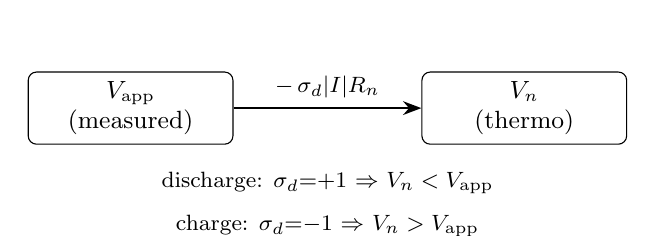
\begin{tikzpicture}[x=1cm,y=1cm,
  box/.style={draw,rounded corners=3pt,minimum width=2.6cm,minimum height=0.9cm,
    align=center,font=\small},
  arr/.style={-{Stealth[scale=1.0]},thick}]
\node[box] (vapp) at (0,0) {$V_\app$ \\ (measured)};
\node[box] (vn)   at (5,0) {$V_n$ \\ (thermo)};
\draw[arr] (vapp) -- (vn) node[midway,above,font=\footnotesize]
  {$-\,\sigma_d|I|R_n$};
\node[font=\footnotesize] at (2.5,-0.95)
  {discharge: $\sigma_d{=}{+1}$ $\Rightarrow$ $V_n < V_\app$};
\node[font=\footnotesize] at (2.5,-1.5)
  {charge: $\sigma_d{=}{-1}$ $\Rightarrow$ $V_n > V_\app$};
\end{tikzpicture}
\caption{분극 변환~\eqref{eq:vn}. 인가 전위 $V_\app$ 에서 방향 부호 $\sigma_d$ 와 분극
저항 $R_n$ 을 곱한 IR 강하를 빼면 열역학 전위 $V_n$ 이 나온다. 이후 모든 평형·속도식은
$V_n$ 을 입력으로 받는다(\texttt{dqdv}, L412).}
\label{fig:polar}
\end{figure}

$V_n$ 을 얻은 뒤 코드는 작업 격자 \texttt{V\_work} 를 $V_n$ 범위의 전후 여유를 포함해
균일하게 구성하고(L419), 배경 기저선 $C_\bg$ 를 격자 위에 초기화한다(L431--L433).
이 격자 위에서 N2$\sim$N8 의 전이별 계산이 수행된다.

% ====================================================================
\section{평형 중심 $U_j(T)$: 열역학에서 전이 전위로 (N2)}\label{sec:Uj}
% ====================================================================

전이별 루프(L435)의 첫 단계는 평형 중심 전위 $U_j(T)$ 를 계산하는 것이다(L437--440).

\subsection{열역학 기초: $\Delta G = -FU$}

등온·등압계에서 삽입 반응
\begin{equation}
\mathrm{Li}^+ + e^- + [\,] \;\rightleftharpoons\; \mathrm{Li}_{(\text{흑연})}
\label{eq:rxn}
\end{equation}
의 자유에너지 변화는 $\Delta G = \Delta H - T\Delta S$ 이고, 전기화학에서 평형 전위와
자유에너지의 관계는:
\begin{equation}
\Delta G_j = -F\,U_j.
\label{eq:gu}
\end{equation}
Gibbs 항등식 $\partial\Delta G/\partial T\big|_P = -\Delta S$ 를 식~\eqref{eq:gu} 에
적용하면 $\partial U_j/\partial T = \Delta S_{\mathrm{rxn},j}/F$ 가 나온다.

\subsection{$U_j(T)$ 의 닫힌 꼴}

$\Delta G_j = \Delta H_{\mathrm{rxn},j} - T\,\Delta S_{\mathrm{rxn},j}$ 를 식~\eqref{eq:gu}
에 넣으면:
\begin{equation}
\boxed{U_j(T) = \frac{-\Delta H_{\mathrm{rxn},j} + T\,\Delta S_{\mathrm{rxn},j}}{F}.}
\label{eq:Uj}
\end{equation}
코드 구현 (\texttt{func\_U\_j}, L68):
\begin{equation*}
\texttt{func\_U\_j}(T,\,\Delta H_{\mathrm{rxn}},\,\Delta S_{\mathrm{rxn}})
= \frac{-\Delta H_{\mathrm{rxn}} + T\,\Delta S_{\mathrm{rxn}}}{F}.
\end{equation*}

\textbf{부호 주의.} $\Delta H_{\mathrm{rxn},j}<0$ (삽입 발열)이면 $-\Delta H_{\mathrm{rxn}}>0$
라 $U_j>0$ — 흑연 음극의 양의 반쪽전지 전위와 정합. $\Delta S_{\mathrm{rxn},j}$
의 온도 의존은 $|\partial U_j/\partial T| = |\Delta S_j|/F \sim 0.01$--$0.1$ mV/K 규모로
작아서 수십 K 창에서 mV 수준 이동을 만든다.

\begin{verifybox}
\texttt{GRAPHITE\_STAGING\_LIT}(L535) 의 stage $4\to3$ 전이:
$\Delta H_{\mathrm{rxn}}=-11700$ J/mol, $\Delta S_{\mathrm{rxn}}=+29$ J/(mol\,K) 이면
$U_j(298) = (11700 + 298\times29)/96485 = (11700+8642)/96485 \approx 0.211$ V,
목표값 $0.210$ V 와 정합.
\end{verifybox}

전이 dict 에 \texttt{'U'} 가 직접 주어지면 코드는 열역학 환산을 우회해 그 값을 사용한다
(L440). 이후 노드 N3 가 이 $U_j$ 에 히스테리시스 이동을 더해 방향별 중심 \texttt{center}
를 결정한다.

% ====================================================================
\section{히스테리시스 분기: 정규용액과 spinodal gap (N3)}\label{sec:hys}
% ====================================================================

N3 는 \textit{방전(본론) 위상}과 \textit{충방전 분기(확장) 위상}을 동시에 처리한다.
$\gamma_j=0$ 이면 분기가 없어 방전 본론으로 직결되고, $\gamma_j>0$ 이면 방·충전
중심이 갈라진다(L448--454).

\subsection{정규용액 자유에너지와 화학퍼텐셜}

$N$ 자리에 Li 가 점유율 $\theta_j = 1-\xi_j$ 로 채워진 계의 자유에너지는 기준·섞임·
상호작용 세 몫으로 나뉜다:
\begin{equation}
\bar{g}_j(\xi) = g_j^0
+ RT\bigl[\xi\ln\xi + (1-\xi)\ln(1-\xi)\bigr]
+ \Omega_j\,\xi(1-\xi).
\label{eq:gxi}
\end{equation}
($\xi_j = 1-\theta_j$ 로 이미 변수 전환함.) 식~\eqref{eq:gxi} 를 $\xi$ 로 미분하면
화학퍼텐셜의 조성 의존이 닫힌다:
\begin{equation}
\mu(\xi) = g_j'(\xi) = RT\ln\frac{\xi}{1-\xi} + \Omega_j(1-2\xi).
\label{eq:mu}
\end{equation}
상호작용 항 $\Omega_j(1-2\xi)$ 가 단조성을 약화시켜, $\Omega_j>2RT$ 이면 식~\eqref{eq:gxi}
가 이중 우물(double well)이 되고 두 상의 공존이 열역학적으로 유리해진다.

\subsection{spinodal 경계와 $\Delta U_j^\hys$}

$g_j''(\xi)=RT/[\xi(1-\xi)]-2\Omega_j=0$ 의 두 근이 spinodal 이다:
\begin{equation}
\xi_{s,j}^\pm = \tfrac{1}{2} \pm \tfrac{1}{2}\,u_j,
\qquad u_j \equiv \sqrt{1 - \frac{2RT}{\Omega_j}}
\qquad (\Omega_j > 2RT).
\label{eq:spinodal}
\end{equation}
두 spinodal 점에서의 평형 전위 차이가 충방전 분기 gap 의 상한이다. 식~\eqref{eq:gxi}
의 1차 미분 $g_j'(\xi) = F(V_{\eq}-U_j)$ 을 $\xi_{s,j}^\pm$ 에 대입하고 차를 구하면:
\begin{equation}
\boxed{\Delta U_j^\hys = \frac{2}{F}\bigl[\Omega_j\,u_j - 2RT\,\mathrm{artanh}\,u_j\bigr].}
\label{eq:dU}
\end{equation}
코드 구현 (\texttt{func\_dU\_hys}, L123--130). $\Omega_j \le 2RT$ 이면 $u_j$ 가 허수라
$\Delta U_j^\hys := 0$ (L127).

\textbf{임계 거동.} $\Omega_j\to 2RT$ ($u_j\to0$) 에서 $\mathrm{artanh}\,u\approx u + u^3/3$
을 전개하면 $\Delta U_j^\hys \propto u_j^3 \propto (T_{c,j}-T)^{3/2}$, $T_{c,j}=\Omega_j/2R$
— gap 이 임계온도에서 부드럽게 소멸한다.

\subsection{방향별 분기 중심}

spinodal 두 점의 평균 전위가 정확히 $U_j$ 임을 확인할 수 있으므로($g'$ 의 반대칭성),
실측 분기는 이 중심에서 $\pm\tfrac{1}{2}\gamma_j\Delta U_j^\hys$ 만큼 갈라진다:
\begin{equation}
U_j^d = U_j + \tfrac{1}{2}\,\sigma_d\,h_\eta\,\gamma_j\,\Delta U_j^\hys.
\label{eq:branch}
\end{equation}
코드 (\texttt{func\_U\_branch}, L133--138; 호출 L451):
\begin{equation*}
\texttt{func\_U\_branch}(T,U_j,\Omega_j,\gamma_j,\sigma_d,h_\eta)
= U_j + \tfrac{1}{2}\,\sigma_d\,h_\eta\,\gamma_j\,\Delta U_j^\hys.
\end{equation*}
방전($\sigma_d=+1$)에서 중심이 위로, 충전($\sigma_d=-1$)에서 아래로 이동한다 —
같은 peak 위치가 방·충전에서 갈리는 이유다.

\begin{verifybox}
$\gamma_j=0$ 이면 $U_j^d = U_j$ — 분기 없음. $\Omega_j \le 2RT$ 이면 $\Delta U_j^\hys=0$
라 역시 $U_j^d=U_j$ — 임계 이하에서 히스테리시스 소멸.
\end{verifybox}

분기 중심 \texttt{center} 는 이후 N4--N6 의 평형 계산 전체에 사용된다.

그림~\ref{fig:hys} 는 정규용액 자유에너지의 이중 우물 구조와 방·충전 과주행 경로를
보여준다.

\begin{figure}[t]
\centering
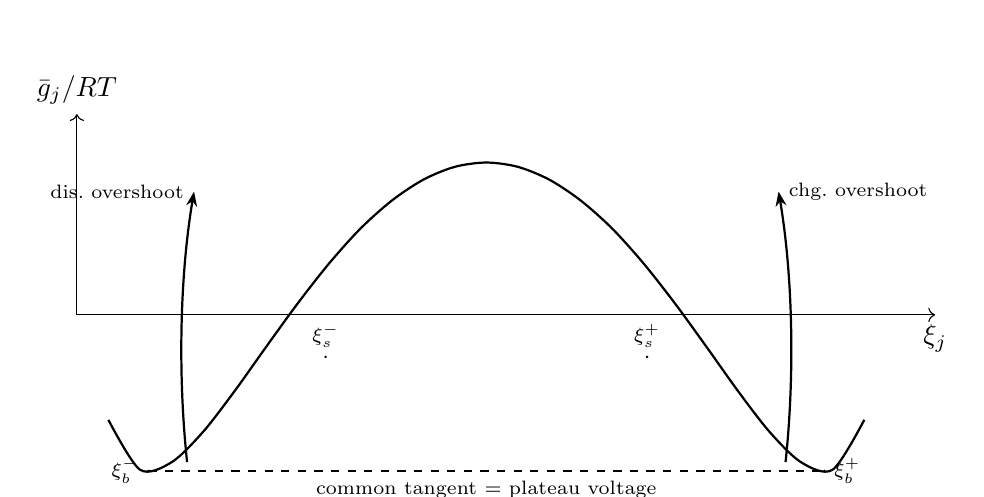
\begin{tikzpicture}[x=10cm,y=34cm]
% Omega=3RT 자유에너지: g(xi) = RT[xi*ln(xi)+(1-xi)*ln(1-xi)] + 3RT*xi*(1-xi)
% 정규화: g/RT, spinodal xi_s^pm = 0.5 +- sqrt(1/6) ~ 0.5 +- 0.2041
\draw[->] (-0.02,0) -- (1.07,0) node[below] {$\xi_j$};
\draw[->] (-0.02,0) -- (-0.02,0.075) node[above] {$\bar{g}_j/RT$};
\draw[thick] plot[smooth] coordinates {
  (0.02,-0.0392)(0.06,-0.0578)(0.10,-0.0551)(0.14,-0.0438)(0.18,-0.0286)
  (0.22,-0.0121)(0.26,0.0041)(0.30,0.0191)(0.34,0.0322)(0.38,0.0427)
  (0.42,0.0505)(0.46,0.0553)(0.50,0.0569)(0.54,0.0553)(0.58,0.0505)
  (0.62,0.0427)(0.66,0.0322)(0.70,0.0191)(0.74,0.0041)(0.78,-0.0121)
  (0.82,-0.0286)(0.86,-0.0438)(0.90,-0.0551)(0.94,-0.0578)(0.98,-0.0392)};
% common tangent (binodal)
\draw[dashed] (0.0707,-0.0583) -- (0.9293,-0.0583)
  node[pos=0.5,below,font=\scriptsize] {common tangent $=$ plateau voltage};
\fill (0.0707,-0.0583) circle (0.5pt) node[left,font=\scriptsize] {$\xi_b^-$};
\fill (0.9293,-0.0583) circle (0.5pt) node[right,font=\scriptsize] {$\xi_b^+$};
% spinodal
\fill (0.2959,-0.0157) circle (0.5pt) node[above,font=\scriptsize] {$\xi_s^-$};
\fill (0.7041,-0.0157) circle (0.5pt) node[above,font=\scriptsize] {$\xi_s^+$};
% arrows: discharge overshoot left, charge overshoot right
\draw[-{Stealth[scale=0.8]},thick] (0.12,-0.055) arc[start angle=200,end angle=150,radius=0.12]
  node[left,font=\scriptsize] {dis.\ overshoot};
\draw[-{Stealth[scale=0.8]},thick] (0.88,-0.055) arc[start angle=-20,end angle=30,radius=0.12]
  node[right,font=\scriptsize] {chg.\ overshoot};
\end{tikzpicture}
\caption{정규용액 자유에너지 $\bar{g}_j(\xi)$ ($\Omega_j=3RT$, 식~\eqref{eq:gxi}).
두 접점 $\xi_b^\pm$(binodal)을 잇는 공통 접선이 plateau 전위를 정한다. 변곡점
$\xi_s^\pm$(spinodal, 식~\eqref{eq:spinodal})이 불안정 구간의 경계다.
방전은 $\xi_s^-$ 까지, 충전은 $\xi_s^+$ 까지 준안정 가지를 과주행하다 분리
점화가 일어나며, 두 과주행 끝점의 전위 차이가 $\Delta U_j^\hys$(식~\eqref{eq:dU}).}
\label{fig:hys}
\end{figure}

% ====================================================================
\section{폭과 평형 점유 (N4, N5)}\label{sec:width}
% ====================================================================

N3 까지 분기 중심 $U_j^d$ 가 결정되면, N4 가 폭 $w_j$ 를 산출하고 N5 가
평형 점유율 $\xi_{\eq,j}$ 를 계산한다.

\subsection{전이 폭 $w_j$ (N4)}

이상 격자기체($\Omega_j=0$)에서 $\xi_{\eq}$ 의 $V_n$ 의존이 logistic 임은 \S\ref{sec:eqpeak}
에서 유도된다. 그 logistic 의 중심 기울기 $\dd\xi/\dd V|_{1/2} = s/(4w)$ 가 폭 척도를
정의하며, 가장 자연스러운 척도는:
\begin{equation}
w_j = \frac{n_j RT}{F}
\label{eq:wj}
\end{equation}
이다(\texttt{func\_w}, L64--65). 이상 극한($n_j=1$)에서 $w=RT/F=25.7$ mV ($25^\circ$C).

상호작용 $\Omega_j>0$ 이면 등온선의 중심 기울기가 줄어 유효 폭이 좁아진다.
두 식~\eqref{eq:wj}·등온선 중심 기울기를 같다고 놓으면:
\begin{equation}
w_j^\eff = \frac{RT}{F}\!\left(1 - \frac{\Omega_j}{2RT}\right)
\label{eq:weff}
\end{equation}
(\texttt{func\_w\_eff}, L141--146). $\Omega_j\to2RT$ 에서 $w^\eff\to0$, $\Omega_j>2RT$
에서 등온선이 비단조가 되어 상분리로 진입한다. 코드 기본 동작은 \texttt{use\_w\_eff=False}
— 식~\eqref{eq:wj} 를 사용하고, \texttt{use\_w\_eff=True} 로 식~\eqref{eq:weff} 를 켠다.

\subsection{평형 점유율 $\xi_{\eq,j}$ (N5)}

정·역 두 방향 반응의 속도 균형(detailed balance)에서 정지점을 구하면 logistic 형이
나온다(N2 $\to$ N5 의 논리 사슬은 \S\ref{sec:eqpeak} 에서 전개):
\begin{equation}
\boxed{\xi_{\eq,j}(V_n,T) = \frac{1}{1+\exp\!\bigl[-\sigma_d(V_n - U_j^d)/w_j\bigr]}.}
\label{eq:ksi}
\end{equation}
코드 (\texttt{func\_ksi\_eq}, L84--87; 호출 L459):
분기 중심 \texttt{center} $= U_j^d$ 와 방향 $\sigma_d$ 를 인자 \texttt{s}(=\texttt{sigma\_d})로 받는다.

\textbf{부호 검산.} 방전($\sigma_d=+1$): $V_n\uparrow$ $\Rightarrow$ 지수 인자 증가 $\Rightarrow$
$\xi_{\eq}\uparrow$ — 전위 상승이 탈리튬화를 촉진. $V_n = U_j^d$ 에서 $\xi_{\eq}=1/2$.

그림~\ref{fig:logistic} 은 $\xi_{\eq}$ 와 그 미분의 형태를 보여준다.

\begin{figure}[t]
\centering
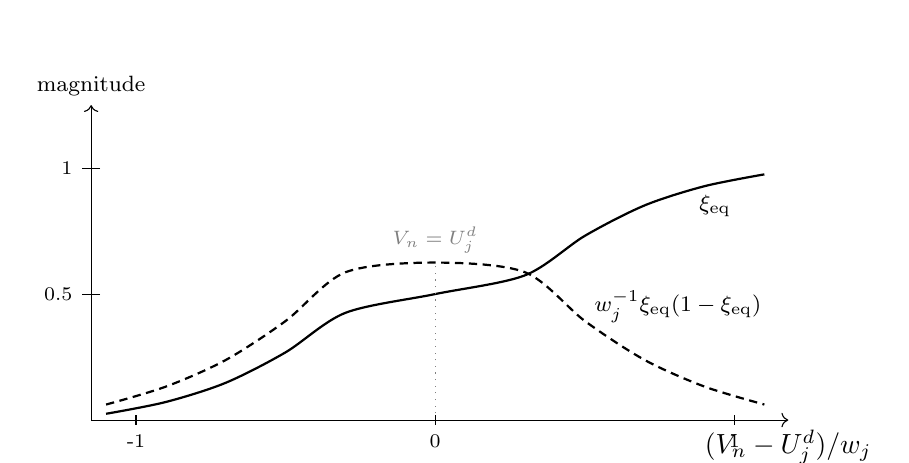
\begin{tikzpicture}[x=3.8cm,y=3.2cm]
\draw[->] (-1.15,0) -- (1.18,0) node[below] {$(V_n-U_j^d)/w_j$};
\draw[->] (-1.15,0) -- (-1.15,1.25) node[above] {\footnotesize magnitude};
% xi_eq = logistic
\draw[thick] plot[smooth] coordinates {
  (-1.1,0.0249)(-0.9,0.0718)(-0.7,0.1480)(-0.5,0.2689)(-0.3,0.4256)
  (0.0,0.5000)(0.3,0.5744)(0.5,0.7311)(0.7,0.8520)(0.9,0.9282)(1.1,0.9751)};
\node[right,font=\footnotesize] at (0.85,0.85) {$\xi_{\eq}$};
% dxi/dV = xi(1-xi)/w — peak at 0, max=0.25 -> 1.25 scaled
\draw[thick,densely dashed] plot[smooth] coordinates {
  (-1.1,0.0616)(-0.9,0.1328)(-0.7,0.2384)(-0.5,0.3932)(-0.3,0.5866)
  (0.0,0.6250)(0.3,0.5866)(0.5,0.3932)(0.7,0.2384)(0.9,0.1328)(1.1,0.0616)};
\node[right,font=\footnotesize] at (0.5,0.45) {$w_j^{-1}\xi_{\eq}(1-\xi_{\eq})$};
\draw[dotted,gray] (0,0)--(0,0.625) node[above,font=\scriptsize] {$V_n=U_j^d$};
\foreach \x in {-1,0,1} {\draw (\x,0.02)--(\x,-0.02) node[below,font=\scriptsize] {\x};}
\foreach \y in {0.5,1} {\draw (-1.12,\y)--(-1.18,\y) node[left,font=\scriptsize] {\y};}
\end{tikzpicture}
\caption{평형 점유율 $\xi_{\eq}$ (실선, 식~\eqref{eq:ksi})과 그 미분
$w_j^{-1}\xi_{\eq}(1-\xi_{\eq})$ (파선, 식~\eqref{eq:dxidV}). 미분이
$V_n=U_j^d$ 에서 $1/(4w_j)$ 의 최댓값을 가지는 종(bell) 모양이며,
이것이 평형 peak 다(\S\ref{sec:eqpeak}). 방향 부호 $\sigma_d=+1$ 기준.}
\label{fig:logistic}
\end{figure}

% ====================================================================
\section{평형 peak: logistic 미분이 만드는 종 모양 (N6)}\label{sec:eqpeak}
% ====================================================================

이 절은 N5 의 $\xi_{\eq}$ 로부터 평형 peak 를 유도한다. 동시에 N5 의 logistic 형이
어디서 오는지를 속도론 관점에서 보인다.

\subsection{속도론에서 logistic 유도}

활성화 자유에너지 $\Delta G_{a,j}$ 를 넘는 확률은 Boltzmann 인자에 비례한다
(Eyring 속도식):
\begin{equation}
k_0 = \frac{k_B T}{h}, \qquad k \simeq k_0\,\exp\!\left[-\frac{\Delta G_a}{RT}\right].
\label{eq:eyring}
\end{equation}
구동력(affinity) $\mathcal{A}_j = \sigma_d F(V_n - U_j)$ 가 정방향 장벽을 $\chi\mathcal{A}_j$
만큼 낮추고 역방향은 $(1-\chi)\mathcal{A}_j$ 만큼 높인다. 자리 점유 인자를 포함하면
운동방정식이:
\begin{equation}
\frac{\dd\xi_j}{\dd t} = r_j^+(1-\xi_j) - r_j^-\xi_j = k_j(\xi_{\eq,j}-\xi_j),
\label{eq:relax}
\end{equation}
정지점($\dd\xi/\dd t=0$)에서 $r_j^+(1-\xi_{\eq})=r_j^-\xi_{\eq}$, detailed balance
$r_j^+/r_j^- = e^{\mathcal{A}_j/RT}$ 를 넣어 $\xi_{\eq}$ 에 대해 풀면 식~\eqref{eq:ksi}
의 logistic 이 나온다. 폭 $w_j=n_jRT/F$ 는 이 도출에서 자연스럽게 등장하는 척도다.

\subsection{$\xi_{\eq}$ 의 미분 — 종 모양}

식~\eqref{eq:ksi} 를 $z=\sigma_d(V_n-U_j^d)/w_j$ 로 치환해 $V_n$ 으로 미분하면:
\begin{equation}
\frac{\dd\xi_{\eq,j}}{\dd V_n}
= \frac{\sigma_d}{w_j}\,\xi_{\eq,j}(1-\xi_{\eq,j}).
\label{eq:dxidV}
\end{equation}
$\xi_{\eq}(1-\xi_{\eq})$ 는 $\xi_{\eq}=1/2$($V_n=U_j^d$)에서 최대 $1/4$ 인 종 모양.
방향 인자 $\sigma_d$ 가 있어 충전($\sigma_d=-1$)에서 $\dd\xi_{\eq}/\dd V_n < 0$
이지만, 코드 L468 은 $\sigma_d$ 없이 \texttt{ksi\_eq*(1.0-ksi\_eq)/w} 를 바로 반환한다.
이는 충전 꼬리 계산(N8) 에서 격자를 역전한 뒤 peak\_shape 를 구성하므로 부호가 자동 양수가 되기 때문이다(아래 검산).

관측 $\dd Q/\dd V$ 는 전하 보존 $Q_\cell\,q = Q_\bg(V_n) + \sum_jQ_j\xi_j$ 를
$V_n$ 으로 미분해 얻는다:
\begin{equation}
\frac{\dd Q}{\dd V_n} = C_\bg + \sum_j Q_j\,\frac{\dd\xi_j}{\dd V_n}.
\label{eq:dQdV}
\end{equation}
평형 추종 극한($\xi_j\to\xi_{\eq,j}$) 에서 식~\eqref{eq:dxidV} 를 넣으면 평형 peak 가:
\begin{equation}
\boxed{
\left.\frac{\dd Q}{\dd V_n}\right|_{\eq}
= C_\bg + \sum_j Q_j\,\frac{\xi_{\eq,j}(1-\xi_{\eq,j})}{w_j}.}
\label{eq:eqpeak}
\end{equation}
코드 L468 의 \texttt{peak\_shape = ksi\_eq*(1.0-ksi\_eq)/w} 가 이 식이다.

\begin{verifybox}
\textbf{peak 세 양.} 위치 $=U_j^d(T)$, 최대 높이 $=Q_j/(4w_j)$, 면적
$\int(\dd Q/\dd V - C_\bg)\dd V = Q_j$ ($\int_0^1\dd\xi=1$).
\textbf{부호.} $\xi(1-\xi)\ge0$ 항상, $w_j>0$ 항상 $\Rightarrow$ 식~\eqref{eq:eqpeak}
의 peak 양수. 충전($\sigma_d=-1$)은 $\dd\xi_{\eq}/\dd V_n<0$ 이지만
N8 격자 역전(\S\ref{sec:tail})이 부호를 양수로 복원한다 — 코드 L468 에
$\sigma_d$ 가 없는 이유.
\end{verifybox}

식~\eqref{eq:eqpeak} 는 $|I|\to0$ 한계, 즉 \texttt{equilibrium()} 메서드(L354)의
수식 표현이다. 전류가 흐를 때의 이탈은 N7--N8 의 동역학 꼬리가 처리한다.

% ====================================================================
\section{동역학 지연 길이 $L_V$ (N7)}\label{sec:lag}
% ====================================================================

C-rate 가 0 이 아니면 $\xi_j$ 가 $\xi_{\eq,j}$ 를 따라가지 못한다. 이 절은
그 지연의 특성 길이를 유도한다.

\subsection{측정축 운동방정식과 $L_{q,j}$}

정전류 방전($\dd q/\dd t = |I|/Q_\cell$)에서 식~\eqref{eq:relax} 를 $\dd q$ 로 나누면:
\begin{equation}
\frac{\dd\xi_j}{\dd q}
= \frac{Q_\cell k_j}{|I|}\,(\xi_{\eq,j}-\xi_j),
\qquad
L_{q,j} = \frac{|I|}{Q_\cell k_j}.
\label{eq:Lq}
\end{equation}
$L_{q,j}$ 는 요구 속도($|I|/Q_\cell$)와 공급 속도($k_j$)의 비로, 세 인자가 모두 이 양을
통해 꼬리에 들어온다: 온도는 $k_j$ 지수 분모에, 전류는 분자에, 전위는 유효 장벽을
통해 $k_j$ 에 새겨진다.

\subsection{Eyring 속도식의 방향별 전개}

꼬리 영역($\mathcal{A}_j\gg RT$)에서 역방향이 무시되므로 $k_j\simeq r_j^+$. 유효
활성화 장벽을 정의하면:
\begin{equation}
\Delta H_{a,j}^\eff = \Delta H_{a,j} - \chi_d\,\Omega_j,
\label{eq:dHeff}
\end{equation}
여기서 방향별 전달 계수(\texttt{func\_chi\_d}, L155--160):
\begin{equation}
\chi_d =
\begin{cases} \chi & \sigma_d \ge 0 \text{ (방전)}\\
1-\chi & \sigma_d < 0 \text{ (충전)}
\end{cases}
\label{eq:chid}
\end{equation}
이다. 깊은 꼬리($\xi_j\to1$: 방전, $\xi_j\to0$: 충전)에서 상호작용 항 $\pm\Omega_j$ 가
활성화 엔탈피에 흡수되어 방향별로 다른 $\chi_d\Omega_j$ 를 만든다.

\subsection{꼬리 컷 affinity $\mathcal{A}$ 와 $L_q$ 계산}

꼬리가 시작하는 컷 지점에서 affinity 를 평가한다(L333--335):
\begin{equation}
\mathcal{A} = \min(z_{\rm cut}\cdot n_j RT,\; \mathcal{A}_{\rm cap} RT),
\label{eq:Acut}
\end{equation}
($z_{\rm cut}=4.357$ 은 $\xi_{\eq}$ 정점의 약 $5\%$ 에 해당하는 컷.) Eyring 식과 방향별
유효 장벽을 결합하면:
\begin{equation}
\ln L_{q,j} = \ln\frac{|I|h}{Q_\cell k_B T} - \ln\left(1+e^{-\mathcal{A}/RT}\right)
+ \frac{\Delta H_{a,j}^\eff - \chi_d\mathcal{A}}{RT} - \frac{\Delta S_{a,j}}{R}.
\label{eq:lnLq}
\end{equation}
코드 (\texttt{func\_L\_q}, L90--97):
식~\eqref{eq:lnLq} 를 그대로 구현한다. 분모의 $T$ 인자 $k_BT/h$ 가 Eyring prefactor.

\textbf{부호 검산.} $\partial\ln L_{q,j}/\partial V_n < 0$ — 전위 상승($\mathcal{A}$ 증가)
이 장벽을 낮춰 $k_j$ 증가, $L_{q,j}$ 감소. 방전 진행 방향에서 전위 올라갈수록 꼬리
짧아진다.

\subsection{전압축 지연 길이 $L_{V,j}$}

$L_{q,j}$ (무차원, 용량축)를 전압축으로 환산하면:
\begin{equation}
L_{V,j} = \left|\frac{\dd V_n}{\dd q}\right|_{q_a}\cdot L_{q,j}.
\label{eq:LV}
\end{equation}
컷 지점 $q_a$ 에서의 OCV 기울기 $|\dd V/\dd q|_{q_a}$ 는 \texttt{dVdq\_qa}(dict 항목)로
주어진다. 코드 L351:
\begin{equation*}
\texttt{L\_V} = |\texttt{dVdq\_qa}|\times L_{q,j}.
\end{equation*}

$L_{V,j}$ 가 격자 간격의 \texttt{min\_lag\_grid\_steps} 배 이상이면 causal lowpass
필터(N8)가 작동하고, 그 미만이면 평형 peak(식~\eqref{eq:eqpeak})으로 직행한다
(L466--468).

% ====================================================================
\section{인과 기억 꼬리와 충전 격자 역전 (N8)}\label{sec:tail}
% ====================================================================

N7 의 $L_{V,j}$ 가 충분히 크면 N8 의 인과 합성곱이 실행된다. 이 절은
그 합성곱의 물리적 유도와 충전 시 격자 역전의 이유를 설명한다.

\subsection{지수 기억 합성곱의 일반해}

식~\eqref{eq:Lq} 의 지연 $r_j=\xi_{\eq,j}-\xi_j$ 를 따로 적으면:
\begin{equation}
\frac{\dd r_j}{\dd q} = \frac{\dd\xi_{\eq,j}}{\dd q} - \frac{r_j}{L_{q,j}}.
\label{eq:dr}
\end{equation}
이 1계 선형 ODE 의 일반해는 적분인자 $e^{q/L_q}$ 로 닫힌다:
\begin{equation}
r_j(q) = r_j(q_0)\,e^{-(q-q_0)/L_{q,j}}
+ \int_{q_0}^{q} e^{-(q-q')/L_{q,j}}\,\frac{\dd\xi_{\eq,j}}{\dd q'}\,\dd q'.
\label{eq:memory}
\end{equation}
지연은 초기 지연의 지수 감쇠와, 과거 평형 목표 변화율을 지수 커널로 가중한
\emph{기억}의 합이다. 계는 용량축에서 $L_{q,j}$ 길이만큼의 최근 과거를 기억한다.

\subsection{이산 구현: causal lowpass 필터}

코드 (\texttt{\_causal\_lowpass}, L100--118) 는 식~\eqref{eq:memory} 의 합성곱을
1계 IIR 지수 필터로 구현한다:
\begin{equation}
\xi_{\rm lagged}[i] = \alpha\,\xi_{\rm lagged}[i-1] + (1-\alpha)\,\xi_{\eq}[i],
\qquad \alpha = e^{-\Delta V/L_{V,j}},
\label{eq:iir}
\end{equation}
여기서 $\Delta V = $ \texttt{grid\_step}(전압 격자 간격). $\alpha$ 가 작을수록
($L_{V,j}$ 작을수록) 추종이 빨라져 $\xi_{\rm lagged}\to\xi_{\eq}$ — 평형 극한으로 복귀.

\subsection{★충전 격자 역전 (L474--477)}

인과 합성곱은 ``진행 방향의 과거'' 를 기억한다.
\begin{itemize}
\item \textbf{방전}($\sigma_d=+1$): 진행 $=$ $V_n$ 증가 방향 $\Rightarrow$ 격자 오름차순 그대로
  식~\eqref{eq:iir} 적용.
\item \textbf{충전}($\sigma_d=-1$): 진행 $=$ $V_n$ 감소 방향 $\Rightarrow$ 격자를 먼저
  뒤집어(\texttt{ksi\_arr[::-1]}) 필터한 뒤 다시 뒤집는다(\texttt{[::-1]}).
\end{itemize}
코드 L474--477:
\begin{quote}\small\texttt{%
if sigma\_d >= 0:\\
\quad occ\_lagged = \_causal\_lowpass(ksi\_arr, grid\_step, lag\_len\_V)\\
else:\\
\quad occ\_lagged = \_causal\_lowpass(ksi\_arr[::-1], grid\_step, lag\_len\_V)[::-1]
}\end{quote}
역전 없이 적용하면 충전 시 ``미래의 기억'' 을 쓰는 인과율 위반이 발생한다.

\subsection{peak shape 계산}

지연된 점유율 $\xi_{\rm lagged}$ 을 구한 뒤 peak shape 을 만든다(L479):
\begin{equation}
\text{peak\_shape} = \frac{\xi_{\eq,j} - \xi_{\rm lagged}}{L_{V,j}}.
\label{eq:peakshape}
\end{equation}
이것이 관측 $\dd Q/\dd V$ 에서 전이 $j$ 가 기여하는 부분이다.

\textbf{$L_{V,j}\to0$ 극한.} $\xi_{\rm lagged}\to\xi_{\eq}$ 이면 식~\eqref{eq:peakshape} 에서
분자$\to0$, $L_{V,j}\to0$ 이지만 비의 극한은 $\xi_{\eq}(1-\xi_{\eq})/w_j$ 로 수렴해
식~\eqref{eq:eqpeak} 평형 peak 가 회복된다(코드 L466--468 가 이 경우를 직접 선택).

그림~\ref{fig:tail} 은 causal lowpass 의 효과와 충전 격자 역전을 도식화한다.

\begin{figure}[t]
\centering
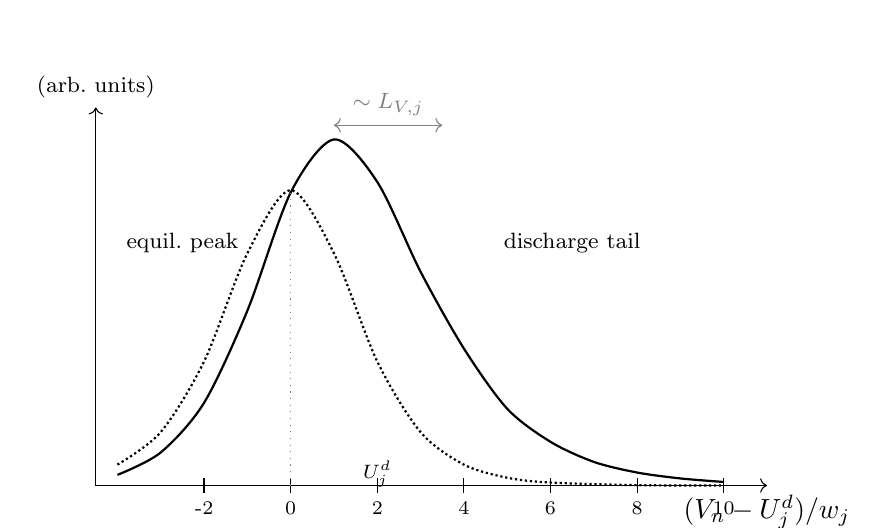
\begin{tikzpicture}[x=0.55cm,y=15cm]
\draw[->] (-4.5,0) -- (11,0) node[below] {$(V_n-U_j^d)/w_j$};
\draw[->] (-4.5,0) -- (-4.5,0.32) node[above] {\footnotesize (arb.\ units)};
\foreach \xx in {-2,0,2,4,6,8,10} {\draw (\xx,0.006)--(\xx,-0.006) node[below,font=\scriptsize] {\xx};}
% equilibrium peak (dotted)
\draw[thick,densely dotted] plot[smooth] coordinates {
  (-4,0.0177)(-3,0.0452)(-2,0.105)(-1,0.1966)(0,0.25)
  (1,0.1966)(2,0.105)(3,0.0452)(4,0.0177)(5,0.0066)(6,0.0025)(8,0.0003)(10,0)};
\node[font=\footnotesize] at (-2.5,0.205) {equil.\ peak};
% discharge tail (solid)
\draw[thick] plot[smooth] coordinates {
  (-4,0.009)(-3,0.028)(-2,0.070)(-1,0.148)(0,0.248)(1,0.293)
  (2,0.257)(3,0.181)(4,0.116)(5,0.065)(6,0.037)(7,0.020)(8,0.011)(9,0.006)(10,0.003)};
\node[font=\footnotesize] at (6.5,0.205) {discharge tail};
% label
\draw[<->,gray] (1,0.305) -- (3.5,0.305) node[pos=0.5,above,font=\footnotesize] {$\sim L_{V,j}$};
\node[font=\scriptsize] at (2,0.01) {$U_j^d$};
\draw[dotted,gray] (0,0)--(0,0.248);
\end{tikzpicture}
\caption{causal lowpass 효과. 점선: 평형 peak($L_{V,j}=0$ 한계, 식~\eqref{eq:eqpeak}).
실선: 유한 $L_{V,j}$ 에서 지연 합성곱 후 peak shape(식~\eqref{eq:peakshape}).
정점이 $\sim L_{V,j}$ 뒤로 이동하고 꼬리가 형성된다.
충전 시에는 격자를 역전(\texttt{[::-1]})하여 필터링해 동일한 양의
\texttt{peak\_shape} 를 만든다(충전 dQ/dV 도 양수 유지).}
\label{fig:tail}
\end{figure}

% ====================================================================
\section{합산과 역보간 (N9)}\label{sec:total}
% ====================================================================

N8 까지 전이별 \texttt{peak\_shape} 가 계산되면 N9 에서 모두 더한다.

\subsection{닫힌 합산식}

작업 격자 위에서(L481):
\begin{equation}
\texttt{dqdv\_work}[V_{\rm work}]
= C_\bg + \sum_{j=1}^{N_p} Q_j \times \texttt{peak\_shape}_j,
\label{eq:sum}
\end{equation}
전이 $j$ 의 기여는 식~\eqref{eq:eqpeak} 또는 식~\eqref{eq:peakshape} 중 하나다.
$C_\bg$ 는 상수 또는 $V$ 함수(\texttt{Cbg}).

\textbf{물리 의미.} 하나의 전이 $j$ 가 주는 peak 는 ``평형 점유율에서 기억이
제거한 부분의 변화율'' 이다:
\begin{equation}
\frac{\dd Q_j}{\dd V_n}\Bigg|_{\rm model}
= Q_j\,\frac{\xi_{\eq,j} - \xi_{\rm lagged,j}}{L_{V,j}}
\;\xrightarrow{L_{V}\to0}\;
Q_j\,\frac{\xi_{\eq,j}(1-\xi_{\eq,j})}{w_j}.
\label{eq:peakfull}
\end{equation}

\subsection{역보간 — 작업 격자에서 $V_n$ 격자로}

\texttt{V\_work} 는 $V_n$ 의 전후 여유를 포함한 균일 격자라서, 결과를 원래 입력
$V_n$ 격자 위로 선형 보간해야 한다(L483):
\begin{equation}
\dd Q/\dd V\big|_{V_n} = \mathrm{interp}(V_n,\; V_{\rm work},\; \texttt{dqdv\_work}).
\label{eq:interp}
\end{equation}
이 보간 결과가 \texttt{dqdv()} 의 반환값이다.

\subsection{staging 4전이 파라미터 (GRAPHITE\_STAGING\_LIT)}

흑연 음극의 4단계 staging 전이($4\to3\to2\mathrm{L}\to2\to1$) 초기값이
\texttt{GRAPHITE\_STAGING\_LIT}(L535--563) 에 정의되어 있다.

\begin{center}
\renewcommand{\arraystretch}{1.3}
\begin{tabular}{ccccccc}
\toprule
전이 & $U$ [V] & $w$ [mV] & $Q/Q_\cell$ & $\Omega$ [J/mol] & $\Delta H_a$ [kJ/mol] & $\Delta V/\Delta q$ \\
\midrule
$4\to3$       & 0.210 & 20 & 0.10 & 6000  & 48 & 0.30 \\
$3\to2\rm{L}$ & 0.140 & 16 & 0.12 & 8000  & 46 & 0.30 \\
$2\rm{L}\to2$ & 0.120 & 14 & 0.25 & 10000 & 44 & 0.30 \\
$2\to1$       & 0.085 & 12 & 0.50 & 13000 & 40 & 0.30 \\
\bottomrule
\end{tabular}
\end{center}
($\Delta H_a$ 는 DFT 활성화 엔탈피 초기값, $\Delta V/\Delta q$ 는 컷 OCV 기울기 \texttt{dVdq\_qa}.
이 값들은 시작점일 뿐 — Optuna 피팅으로 override 된다.)

그림~\ref{fig:full} 은 전체 N0$\to$N9 진행을 한눈에 보여주는 흐름도다.

\begin{figure}[t]
\centering
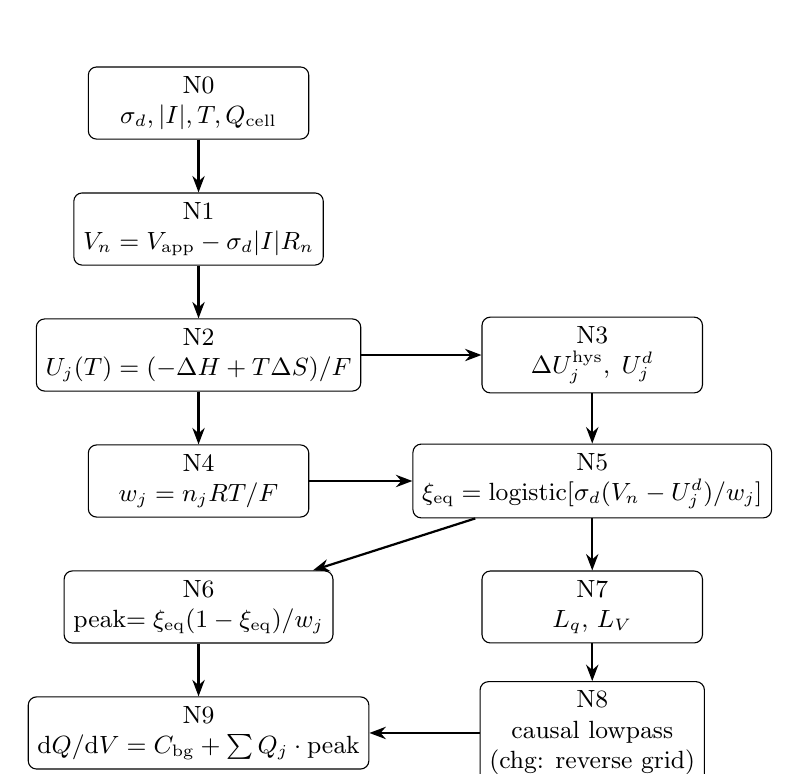
\begin{tikzpicture}[
  box/.style={draw,rounded corners=3pt,minimum width=2.8cm,minimum height=0.85cm,
    align=center,font=\small},
  arr/.style={-{Stealth[scale=0.9]},thick},
  x=1cm,y=1cm]
\node[box] (n0) at (0,0)    {N0\\$\sigma_d,|I|,T,Q_\cell$};
\node[box] (n1) at (0,-1.6) {N1\\$V_n = V_\app - \sigma_d|I|R_n$};
\node[box] (n2) at (0,-3.2) {N2\\$U_j(T)=(-\Delta H+T\Delta S)/F$};
\node[box] (n3) at (5,-3.2) {N3\\$\Delta U_j^\hys,\; U_j^d$};
\node[box] (n4) at (0,-4.8) {N4\\$w_j = n_jRT/F$};
\node[box] (n5) at (5,-4.8) {N5\\$\xi_{\eq}=\mathrm{logistic}[\sigma_d(V_n-U_j^d)/w_j]$};
\node[box] (n6) at (0,-6.4) {N6\\peak$=\xi_{\eq}(1-\xi_{\eq})/w_j$};
\node[box] (n7) at (5,-6.4) {N7\\$L_q,\, L_V$};
\node[box] (n8) at (5,-8.0) {N8\\causal lowpass\\(chg: reverse grid)};
\node[box] (n9) at (0,-8.0) {N9\\$\dd Q/\dd V = C_\bg+\sum Q_j\cdot\text{peak}$};
\draw[arr] (n0)--(n1);
\draw[arr] (n1)--(n2);
\draw[arr] (n2)--(n3);
\draw[arr] (n2)--(n4);
\draw[arr] (n3)--(n5);
\draw[arr] (n4)--(n5);
\draw[arr] (n5)--(n6);
\draw[arr] (n5)--(n7);
\draw[arr] (n6)--(n9);
\draw[arr] (n7)--(n8);
\draw[arr] (n8)--(n9);
\end{tikzpicture}
\caption{v11\_final 코드 진행 N0$\to$N9 의 전체 흐름. 왼쪽 열이 본론(방전·평형),
오른쪽 열이 확장(히스·동역학). 두 열이 N5 에서 만나고 N9 에서 합산된다.
각 노드의 수식은 해당 절에서 유도된다.}
\label{fig:full}
\end{figure}

% ====================================================================
\section{부호 체크리스트 종합}\label{sec:sign}
% ====================================================================

AUTHOR\_BRIEF §8 의 8개 부호 조건을 본문 전개와 대조해 최종 확인한다.

\begin{enumerate}
\item $U_j(T)=(-\Delta H_{\mathrm{rxn}}+T\Delta S_{\mathrm{rxn}})/F$ (식~\eqref{eq:Uj}):
  $\Delta H<0$ 발열이면 $U_j>0$ $\checkmark$, $\Delta G=-FU_j$ 로부터 유도.
\item $\xi_{\eq}=\mathrm{logistic}[\sigma_d(V_n-U_j^d)/w_j]$ (식~\eqref{eq:ksi}):
  방전($\sigma_d=+1$)에서 $V_n\uparrow\Rightarrow\xi_{\eq}\uparrow$ $\checkmark$.
\item $\dd\xi_{\eq}/\dd V_n = \sigma_d\,\xi_{\eq}(1-\xi_{\eq})/w_j$ (식~\eqref{eq:dxidV}):
  충전에서 이 값이 음수지만, 코드 L468 평형 peak 는 $\sigma_d$ 없이
  $\xi_{\eq}(1-\xi_{\eq})/w_j\ge0$ 만 반환. N8 격자 역전(\S\ref{sec:tail})이
  충전 peak 를 양수로 보장 $\checkmark$.
\item $\Delta U_j^\hys\ge0$, $\Omega_j\le2RT\Rightarrow\Delta U_j^\hys=0$ (식~\eqref{eq:dU}) $\checkmark$.
  분기 중심 방전 위로, 충전 아래로 ($\sigma_d$ 부호).
\item $\chi_d$: 방전 $\chi$ / 충전 $1-\chi$ (식~\eqref{eq:chid}).
  $\Delta H_a^\eff=\Delta H_a-\chi_d\Omega_j$ (식~\eqref{eq:dHeff}) $\checkmark$.
\item $\partial\ln L_{q,j}/\partial V < 0$: 식~\eqref{eq:lnLq} 에서
  $\partial\ln L_q/\partial\mathcal{A}=-\chi_d/RT<0$, $\mathcal{A}\propto\sigma_dF(V_n-U_j^d)>0$ 증가 $\checkmark$.
\item 충전 격자 역전(\texttt{ksi\_arr[::-1]$\ldots$[::-1]}, L474--477):
  충전 진행 방향($V_n\downarrow$)이 방전과 반대 — 격자 역전 없이 필터하면
  미래를 보게 된다(인과율 위반). 역전 후 충전 $\dd Q/\dd V>0$ 유지 $\checkmark$.
\item 분극 부호 $V_n=V_\app-\sigma_d|I|R_n$ (식~\eqref{eq:vn}) $\checkmark$.
\end{enumerate}

% ====================================================================
\section{피팅 실행력 (G-usable) — 코드 재현을 위한 요약}\label{sec:fit}
% ====================================================================

이 절만 보고 v11 곡선을 재현할 수 있어야 한다는 선언의 검증이다.

\subsection{한 줄 평가 순서}

입력: $(V_\app,\,\sigma_d,\,|I|,\,Q_\cell,\,T,\,\{$전이 dict$\})$

\begin{enumerate}[label=\textbf{S\arabic*.},leftmargin=2.2em,itemsep=2pt]
\item $V_n = V_\app - \sigma_d|I|R_n$ (N1, 식~\eqref{eq:vn}).
\item $V_{\rm work}$ 균일 격자 구성 (여유 $0.15\times$ span 전후).
\item 전이 $j$ 마다:
  \begin{enumerate}[label=(\alph*),itemsep=0pt]
  \item $U_j(T)$ 계산 (N2, 식~\eqref{eq:Uj} 또는 dict \texttt{'U'}).
  \item $\Delta U_j^\hys$, $U_j^d$ (N3, 식~\eqref{eq:dU}·\eqref{eq:branch}).
  \item $w_j$ (N4, 식~\eqref{eq:wj}).
  \item $\xi_{\eq,j}$ on $V_{\rm work}$ (N5, 식~\eqref{eq:ksi}).
  \item $L_{q,j}$, $L_{V,j}$ (N7, 식~\eqref{eq:lnLq}·\eqref{eq:LV}).
  \item If $L_{V,j} < L_{\rm min}$: peak $=\xi_{\eq}(1-\xi_{\eq})/w_j$ (N6).\\
        Else: \texttt{causal\_lowpass} $\pm$ 역전 $\to$ peak $=(\xi_{\eq}-\xi_{\rm lag})/L_V$ (N8, 식~\eqref{eq:peakshape}).
  \item \texttt{dqdv\_work} $+= Q_j\times$ peak (N9, 식~\eqref{eq:sum}).
  \end{enumerate}
\item $\dd Q/\dd V = \mathrm{interp}(V_n, V_{\rm work}, \texttt{dqdv\_work})$ (식~\eqref{eq:interp}).
\end{enumerate}

\subsection{초기값 및 진단 기준}

전이 초기값: \texttt{GRAPHITE\_STAGING\_LIT} (L535, 본 문서 \S\ref{sec:total} 표).
피팅 순서: $\{U_j,w_j,Q_j\}$ (저율 OCV) $\to$ $R_n$ (전류 차단) $\to$ $\chi$ (다전위 꼬리)
$\to$ $\Delta H_a^\eff$ (다온도 Arrhenius) $\to$ $\{\Omega_j,\gamma_j\}$ (gap 분해).

\subsection{검증 조건}

\begin{itemize}
\item $|I|\to0$: peak $\to\xi_{\eq}(1-\xi_{\eq})/w_j$ (N6 직행).
\item $\gamma_j=0$: 방·충전 peak 중심 일치.
\item $\Omega_j\le2RT$: $\Delta U_j^\hys=0$, 히스테리시스 소멸.
\item 충전 peak 부호: \texttt{peak\_shape}$\ge0$ 항상 (격자 역전으로 보장).
\end{itemize}

% ====================================================================
\begin{thebibliography}{99}
\bibitem{dahn1991} J.~R.~Dahn, ``Phase diagram of Li$_x$C$_6$,''
  \emph{Phys. Rev. B} \textbf{44}, 9170 (1991).
\bibitem{eyring1935} H.~Eyring, ``The Activated Complex in Chemical Reactions,''
  \emph{J. Chem. Phys.} \textbf{3}, 107 (1935).
\bibitem{bazant2013} M.~Z.~Bazant, ``Theory of Chemical Kinetics and Charge Transfer,''
  \emph{Acc. Chem. Res.} \textbf{46}, 1144 (2013).
\bibitem{marcus1956} R.~A.~Marcus, ``On the Theory of Oxidation-Reduction Reactions,''
  \emph{J. Chem. Phys.} \textbf{24}, 966 (1956).
\bibitem{mckinnon1983} W.~R.~McKinnon, R.~R.~Haering,
  in \emph{Modern Aspects of Electrochemistry} \textbf{15}, 235 (1983).
\bibitem{dreyer2010} W.~Dreyer \emph{et al.}, ``The thermodynamic origin of hysteresis,''
  \emph{Nat. Mater.} \textbf{9}, 448 (2010).
\bibitem{reynier2004} Y.~Reynier, R.~Yazami, B.~Fultz,
  \emph{J. Electrochem. Soc.} \textbf{151}, A422 (2004).
\end{thebibliography}

\end{document}
